
\section{Rozdział Chrzest jako narodziny Polski}

\subsection{Wprowadzenie: Narodziny Polski i symboliczna data chrztu}

\begin{figure}

    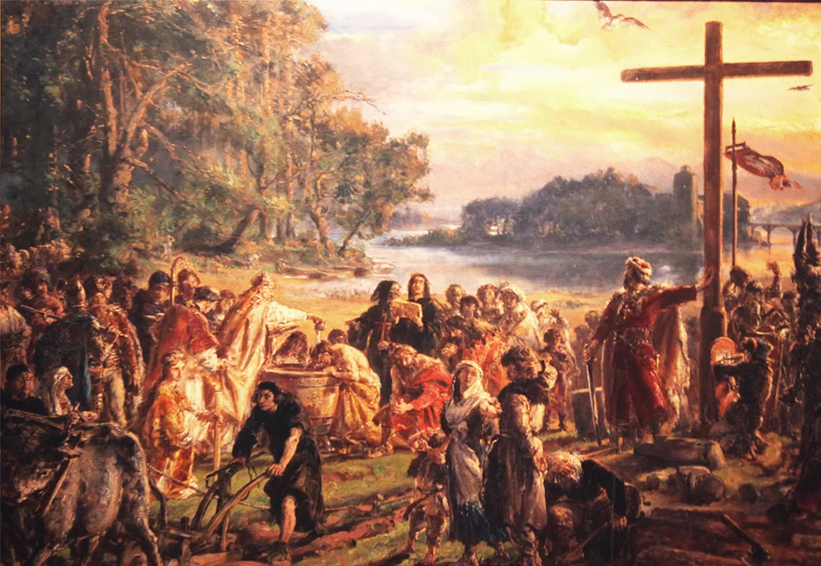
\includegraphics[width=8cm, height=8cm]{Polska_poczatek.png}
\end{figure}

„Każdy Polak powinien być świadomy, jak Polska się narodziła, kiedy i w jakich okolicznościach. Symboliczną datą powstania Polski jako państwa chrześcijańskiego jest rok 966, kiedy Mieszko I przyjął chrzest. Jak zauważa dr hab. Grzegorz Pac, średniowieczne źródła dotyczące tego wydarzenia są skromne i historycy niejednokrotnie muszą opierać się na domysłach i przypuszczeniach.

Niemniej jednak, pewnym faktem jest przyjęcie chrztu przez Mieszka I, które miało fundamentalne znaczenie dla kształtowania tożsamości i charakteru narodu polskiego. Chrzest Polski oznaczał nie tylko włączenie młodego państwa do wspólnoty chrześcijańskich narodów Europy, ale także zapoczątkowanie przemian w strukturze społecznej i prawnej, opartych na wartościach chrześcijańskich.”

\subsection{Przyczyny chrztu i jego znaczenie polityczne}

Decyzja Mieszka I o przyjęciu chrztu miała nie tylko charakter religijny, ale również polityczny. Przyjęcie chrześcijaństwa umożliwiło Polsce zbliżenie się do chrześcijańskiej Europy i zawiązanie sojuszy, co miało kluczowe znaczenie dla stabilizacji i bezpieczeństwa nowo powstałego państwa. Mieszko mógł w ten sposób poślubić księżniczkę Dobrawę, córkę księcia czeskiego, co umocniło pozycję Polski na arenie międzynarodowej i zapewniło jej ochronę przed atakami ze strony pogan. Jednakże jak zauważył dr. hab. Pac konwersja tamtego społeczeństwa z pogańskiego na chrześcijański wymagał silnego władcy, który był w stanie narzucić nowe prawo oparte o wartości i etykę chrześcijańską. W przeciwnym razie doszłoby do podziału społeczeństwa na dwie grupy, które by żyły według dwóch różnych porządków. co prowadziłoby do chaosu i konfliktów wewnętrznych. Lud musiał pójść w ślady za swym władcą, aby mógł zapanować porządek i jedność. Chrystianizacja Polski przebiegała powoli, ale zdecydowanie.

\subsection{Chrystianizacja Polski i jej wpływ na tożsamość narodową}

Chrzest Mieszka I, zwany również „Chrztem Polski”, nadał nowopowstałemu państwu charakter wyznaniowy. Wydarzenie to odcisnęło ponadczasowe piętno na Polsce i jej narodzie, łącząc go nierozerwalnie z chrześcijaństwem i jego dziedzictwem. W kolejnych stuleciach chrześcijaństwo kształtowało etykę, kulturę, światopogląd oraz tradycję Polek i Polaków. Jak ujął to papież Jan Paweł II:
„Chrzest Polski, który dokonał się w 966 roku, jest faktem o fundamentalnym znaczeniu w historii naszego narodu, w jego kulturze, w jego tożsamości, w jego przynależności do chrześcijaństwa. Mieszko I, w tym wielkim akcie, nie tylko wprowadził Polskę do rodziny narodów chrześcijańskich, ale równocześnie nadał narodowi polskiemu charakter, który przez wieki, przez wieki będzie w sposób nieodwracalny stanowił o jego tożsamości.”


